%!TEX root = ../thesis.tex
%*******************************************************************************
%****************************** Third Chapter **********************************
%*******************************************************************************

\chapter{Risultati sperimentali}
\hspace{0,5cm} 


\section{Classificazione con il lessico Hurtlex}
I primi risultati ottenuti sono relativi alla classificazione con il lessico Hurtlex. Il lessico, composto da quasi 7000 lemmi molti dei quali inclusivi, riesce solo in parte a classificare correttamente i commenti in base alla loro categoria di appartenenza. Vengono quindi svolte alcune operazioni in grado di mitigare, anche se solo parzialmente, questo problema.

\subsection{Distribuzione delle categorie ed esempi descrittivi}
    Come descritto precedentemente ogni lemma contenuto nel lessico appartiene a una o più categorie. Tra le 17 categorie quella che ha una frequenza maggiore è quella relativa a \textit{parole dispregiative} seguita da termini relativi alla categoria \textit{omosessualità}. Tutte le altre categorie mantengono una frequenza che si attesta sullo stesso livello.
    
    Osservando i commenti, nello specifico quelli che presentano più segnalazioni, è possibile notare come il lavoro svolto dalla classificazione con il lessico Hurtlex non sia molto efficace nel trovare commenti con un senso offensivo. Nella maggior parte dei casi è possibile trovare commenti che contengono parole considerate offensive dal lessico ma che nella realtà sono applicate ad un contesto totalmente diverso da quello atteso. I falsi positivi risultano quindi essere gran parte dell'output prodotto dalla classificazione con il lessico Hurtlex. 
    
    Di seguito vengono riportati degli esempi esplicativi su quanto affermato in precedenza:
    nel commento "\textit{Sono cretina perché ancora non ti seguivo PS ti adoro}" il lemma segnalato è \textit{cretina} mentre invece in "\textit{sei bravissima e adoro il tuo stile faccio hip hop anche io, vorrei un sacco averti come insegnante ahaha}" viene sengalato il lemma \textit{insegnante}; in entrambi i casi però i commenti risultano essere totalmente inoffensivi.


\subsection{Distinzione tra lemmi conservativi e inclusivi}
    
    Per cercare di arginare il problema relativo alla segnalazione di commenti inoffensivi si è provato ad eseguire l'algoritmo di classificazione sfruttando solamente i termini conservativi che, a differenza dei termini inclusivi, assumono nella maggior parte dei contesti significati prettamente offensivi. In questo caso il numero di commenti segnalati è più basso rispetto alla classificazione precedente come osservabile dal grafico in figura \ref{fig:comments_distribution_conservative_barplot}.
    
    \begin{figure}[h]
        \centering
        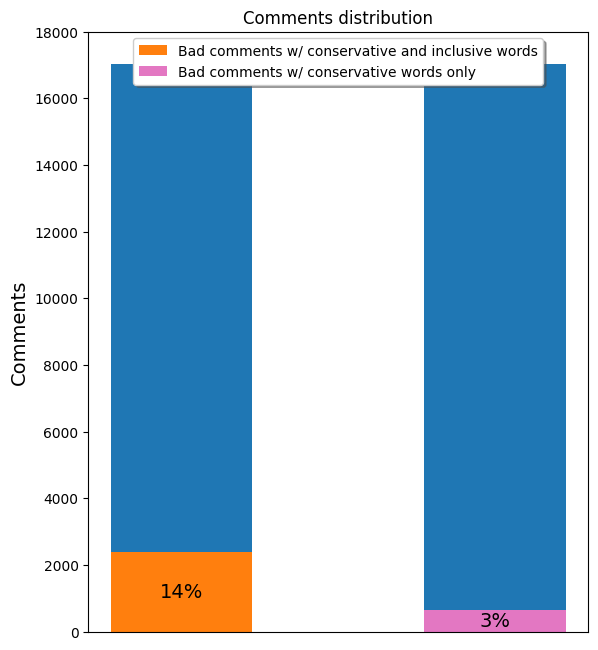
\includegraphics[width=0.5\textwidth]{pics/comments distribution conservative.png}
        \caption{Distribuzione dei commenti classificati come negativi usando lemmi conservativi e inclusivi o esclusivamente lemmi conservativi}
        \label{fig:comments_distribution_conservative_barplot}
    \end{figure}
    
    Nonostante l'utilizzo di lemmi solamente conservativi, la classificazione con il lessico non risulta comunque in grado di separare efficacemente i commenti offensivi da quelli innocui. I commenti segnalati quindi sono del tutto simili a quelli visti negli esempi precedenti. \\
    Dopo una veloce ispezione visiva dei commenti in output è possibile notare come, nonostante vengano selezionati commenti con parole offensive, spesso il contesto cambia il senso della frase. In altri casi invece i lemmi classificati come conservativi non hanno molto a che fare con contesti di offesa come è evidente da alcuni esempi che seguono: "\textit{Io sono due persone diverse praticamente}" e "\textit{Ma adesso che sono chiuse le discoteche come fai a lavorare? (Sembra una domanda aggressiva, ma sono solo curiosa)}" sono stati segnalati per la presenza del lemma \textit{diverso} nel primo commento e \textit{curioso} nel secondo.\\
    Inoltre è importante indicare come i commenti di difesa verso il/la creator di contenuti su TikTok vengano comunque segnalati come offensivi: nel commento "\textit{Ma che cafoni ignoranti! Sei bellissima!}" la presenza dei lemmi \textit{cafone} e \textit{ignorante} classifica automaticamente lo stesso come potenzialmente denigratorio.
    
    In generale, tra tutti i commenti segnalati, sono sicuramente presenti dei commenti offensivi ma, nonostante questo, il numero di falsi positivi rende la classificazione con il lessico Hurtlex poco efficace nell'isolare solamente i commenti negativi.
    




\section{Analisi esplorativa dei dati}
Una volta ottenuto un semplice metodo di classificazione dei commenti è possibile esplorare superficialmente le informazioni raccolte per riassumerne le principali caratteristiche. La numerosità del dataset complessivo supera i 250 000 elementi e, per ognuno, sono state registrate non solo le informazioni relative al corpo del commento ma anche i relativi metadati come le informazioni di base sul profilo proprietario e la data di pubblicazione dello stesso. Di seguito vengono quindi analizzati questi aspetti utili ad avere un quadro più chiaro sui dati a disposizione.

\subsection{Analisi di genere e movimenti temporali}
    
    Una prima considerazione viene svolta sulla distribuzione di genere di chi commenta. TikTok purtroppo non rende pubbliche le informazioni relative all'identificazione di genere di un account ed è stato quindi necessario classificare manualmente un campione di circa 10 000 account presi casualmente in base alla loro immagine profilo e ai contenuti caricati sulla piattaforma. La distribuzione risultante dall'analisi è osservabile nel grafico in figura \ref{fig:gendere distribution} dove è evidente come la presenza femminile sia di molto superiore rispetto alla controparte maschile.
    
    \begin{figure}[h]
        \centering
        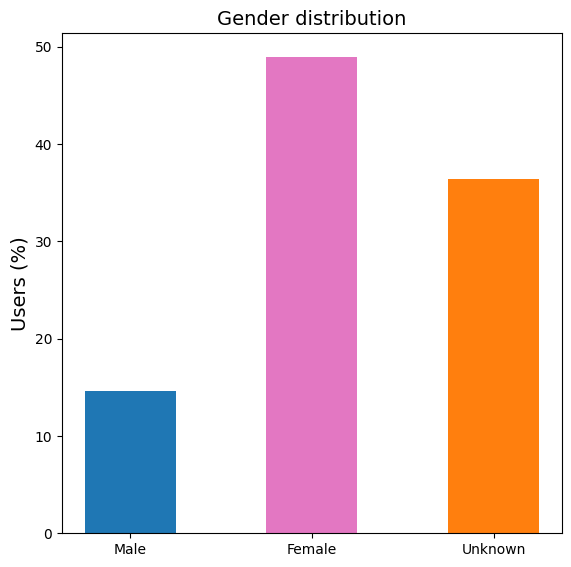
\includegraphics[width=0.5\textwidth]{pics/gender-distribution.png}
        \caption{Distribuzione di genere di un campione di 10 000 account}
        \label{fig:gendere distribution}
    \end{figure}
    
    
    Viene ulteriormente considerata la quantità di commenti segnalati durante il corso del tempo. Dopo aver collegato ogni commento al relativo post di appartenenza e conseguentemente diviso i dati in 10 regioni temporali, è stato possibile notare come la presenza di commenti negativi per ogni account si concentri sopratutto in presenza di post controversi che, diventando virali, attirano nuovi utenti che commentano negativamente. I picchi relativi a questo fenomeno sono osservabili nella figura \ref{fig:bins_total} suddivisi per i quattro account più popolari analizzati.
    
    \begin{figure}[h]
        \centering
        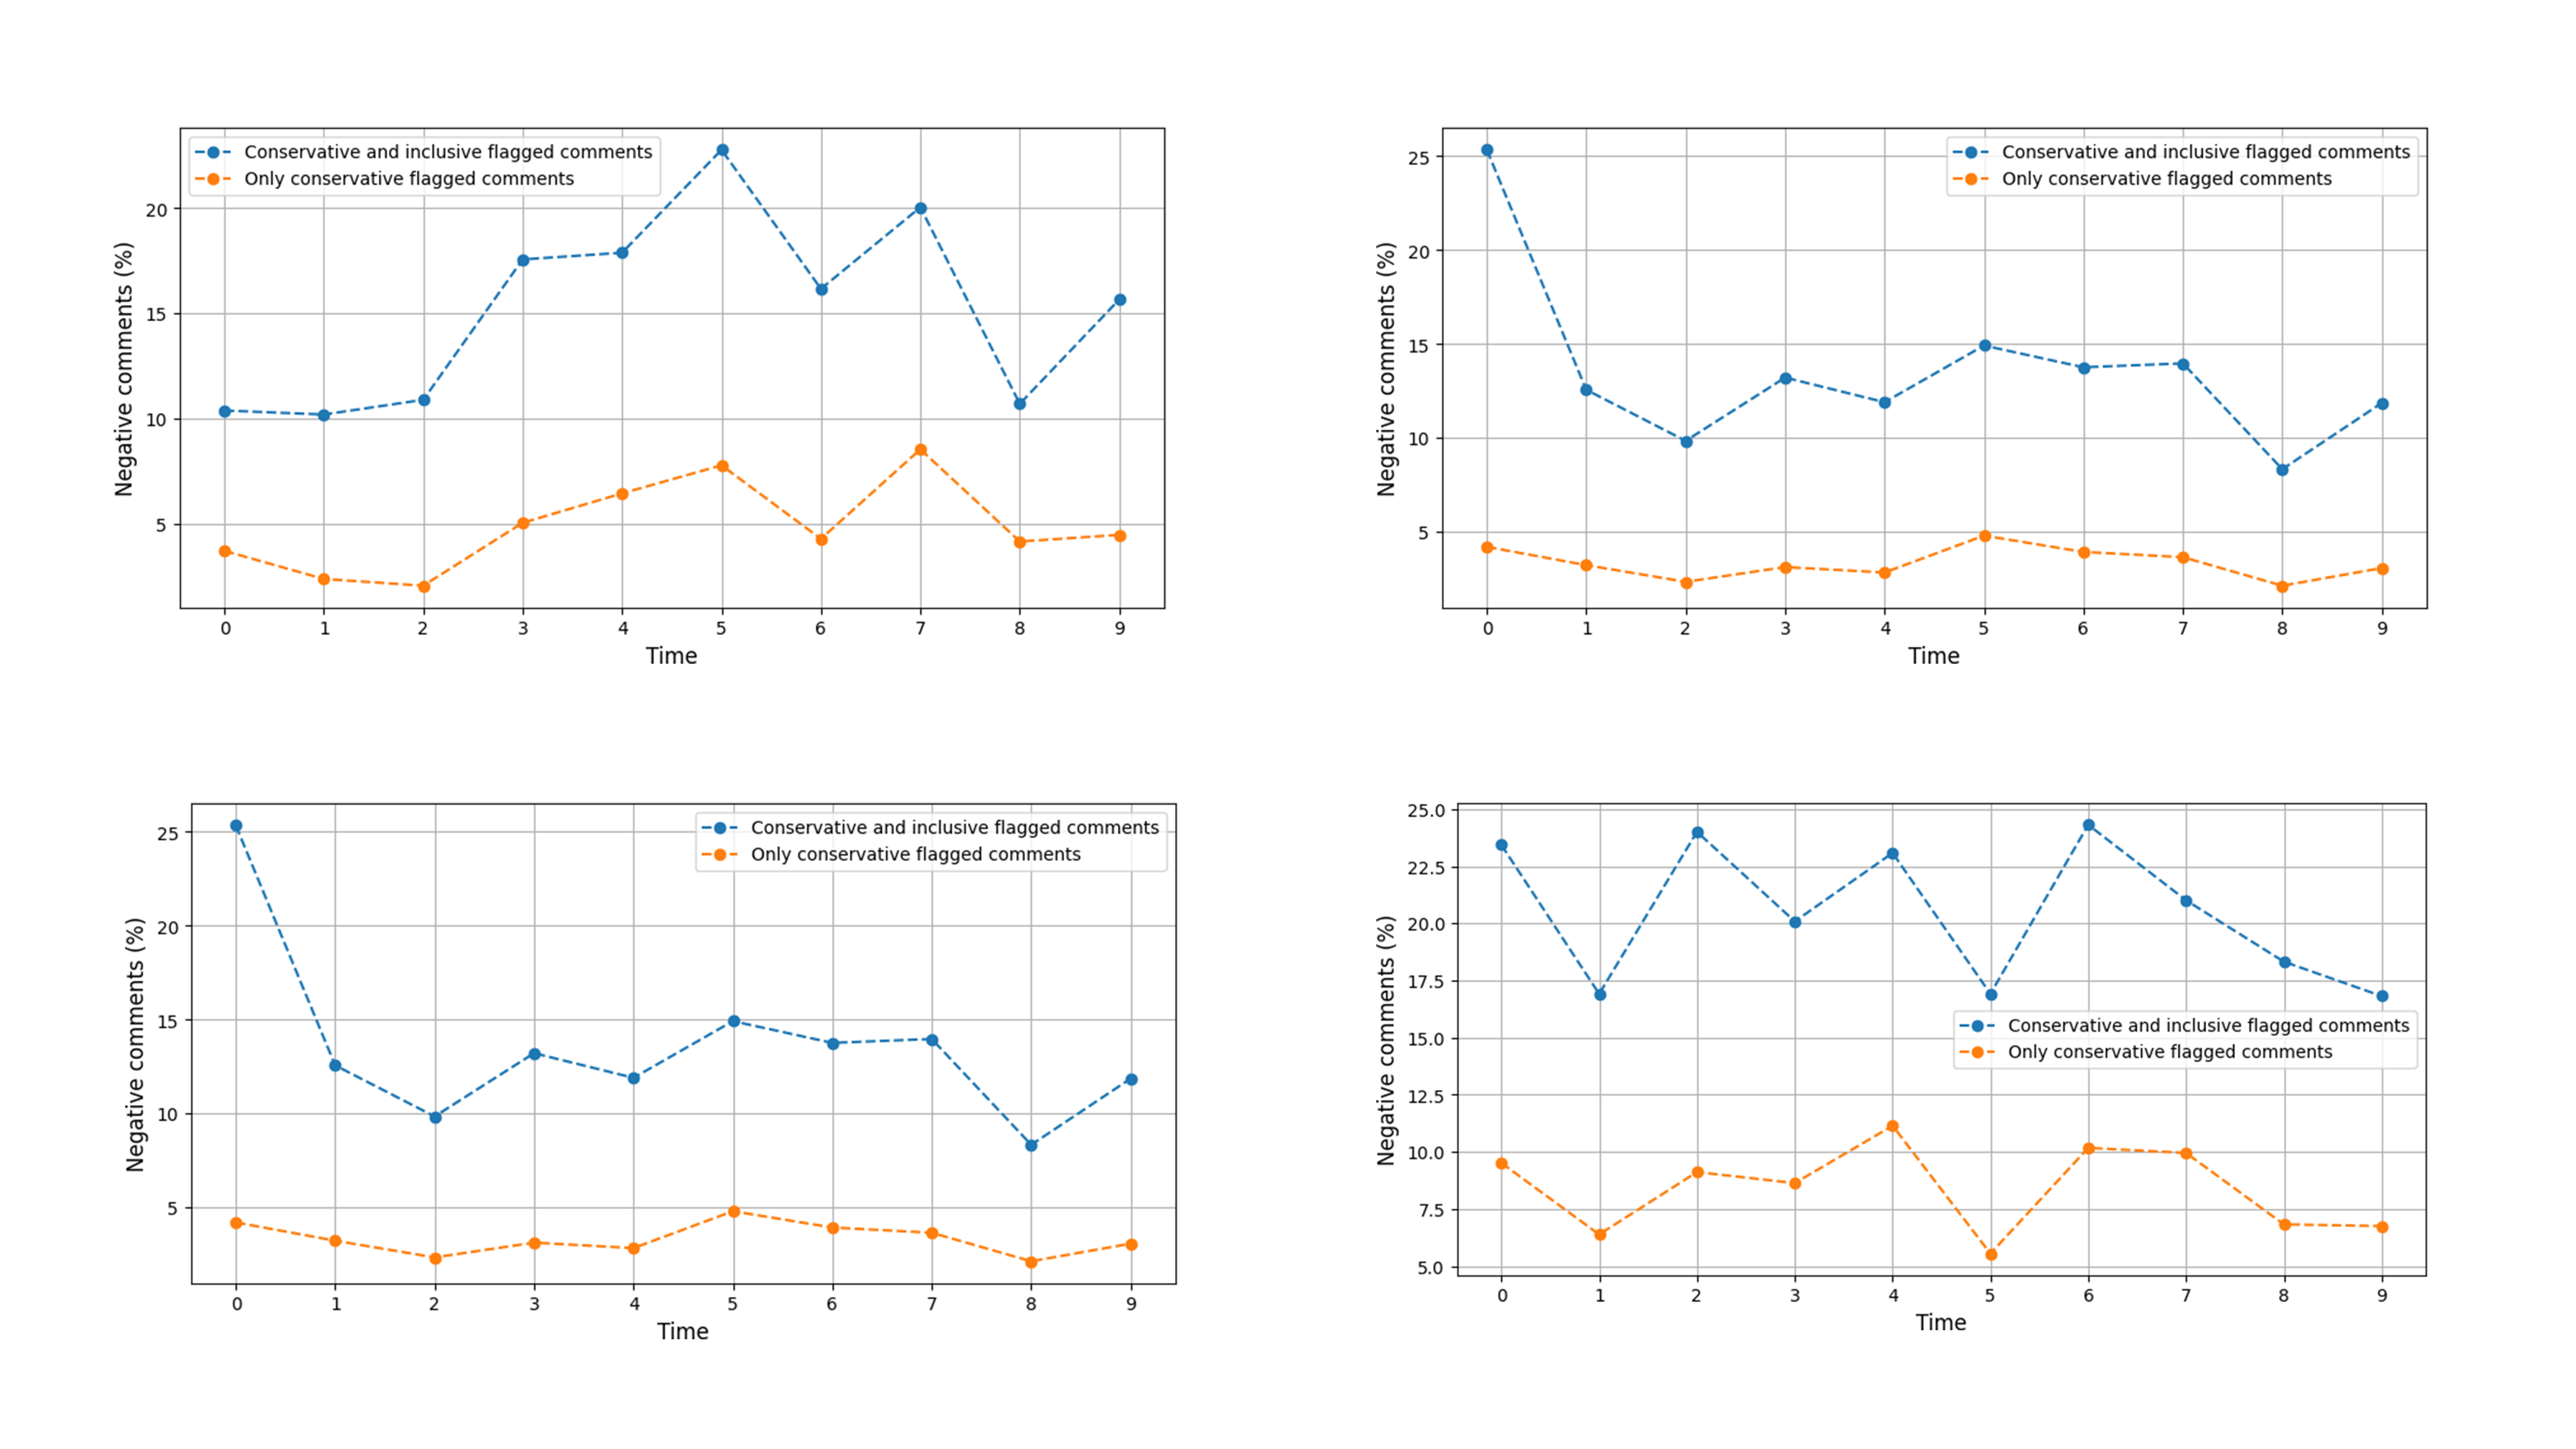
\includegraphics[width=1\textwidth]{pics/bins_comment-total.png}
        \caption{Movimenti temporali dei quattro account più popolari analizzati}
        \label{fig:bins_total}
    \end{figure}





\section{Fine tuning del modello BERT base}
Vengono proposti di seguito i risultati ottenuti dal processo di fine tuning dei modelli BERT descritti nel capitolo relativo al framework proposto. Per misurare la performance dei modelli e delle ottimizzazioni effettuate durante la fase di addestramento viene considerato l'output della funzione \textit{cross-entropia}, una funzione obiettivo (\textit{loss function}) che permette di avere una rappresentazione efficace sullo stato di apprendimento del modello. In seguito, per ogni epoca di addestramento effettuata, vengono considerate metriche quali F1, precisione e recupero osservando le rispettive matrici di confusione. L'accuratezza dei modelli non viene considerata ai fini della descrizione delle performance visto l'impiego di un dataset sbilanciato per la fase di addestramento e di test.


\subsection{Valutazione della funzione obiettivo}
    La valutazione della funzione obiettivo durante la fase di addestramento è essenziale per comprendere come il modello sta apprendendo le informazioni dai dataset di train e di test. Osservando i dati in output è possibile stabilire se la rete neurale si adatta eccessivamente ai dati di train. Questo fenomeno è definito come overfitting e può portare a basse performance per il dataset di test mantenendo allo stesso tempo delle ottime performance nel dataset di addestramento.
    
    La prima fase di test è stata effettuata variando lievemente i parametri consigliati dagli autori dei modelli basati su BERT per cercare quale configurazione di adattasse al meglio al task di classificazione considerato. Il training consiste in otto epoche totali dove, per ogni epoca, viene registrato l'output della loss function sia sul dataset di train che su quello di test. Viene inoltre considerata anche la lunghezza di un singolo batch facendola variare tra 16, 32 e 64. I risultati del primo modello \textit{BERT base italian uncased} vengono mostrati in figura \ref{fig:losses-uncased}.
    
    \begin{figure}[h]
        \centering
        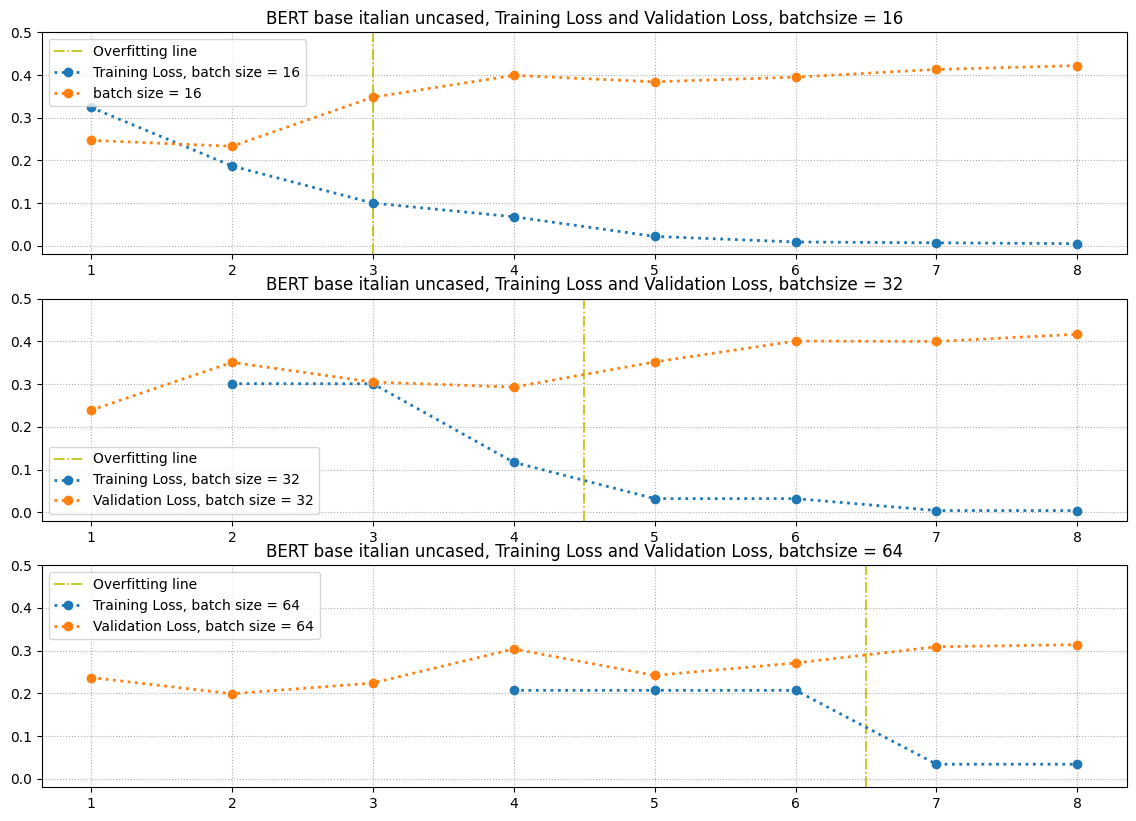
\includegraphics[width=0.65\textwidth]{pics/bert base italian uncased/losses.png}
        \caption{BERT base italian uncased; risultati funzione obiettivo per il dataset di train e di test}
        \label{fig:losses-uncased}
    \end{figure}
    
    
    I grafici ottenuti sono suddivisi secondo la lunghezza del batch utilizzata nella fase di addestramento. Come si può notare, osservando la crescita della funzione obiettivo per il dataset di test e la decrescita della stessa per il dataset di train, la probabilità di overfitting aumenta considerevolmente con l'aumentare delle epoche. Viene quindi rappresentata, attraverso l'utilizzo di una linea gialla, il limite entro il quale è consigliabile rimanere per il numero di epoche di addestramento necessarie al modello prima di incorrere in problemi di overfitting. I parametri ottimi ottenuti coincidono perfettamente con quelli consigliati dagli autori che suggeriscono un numero di epoche comprese nell'intorno di 4.
    
    
    \hspace{0,5cm}
    
    Il secondo modello utilizzato è \textit{BERT base italian xxl cased}. A differenza del modello visto precedentemente viene utilizzato un corpus maggiore nella fase di pre-training (un incremento di circa il 17\%) e viene aggiunta la capacità di riconoscere i caratteri minuscoli da quelli maiuscoli. L'output della funzione obiettivo è rappresentata in figura \ref{fig:losses-xxl}.
    
    \begin{figure}[h]
        \centering
        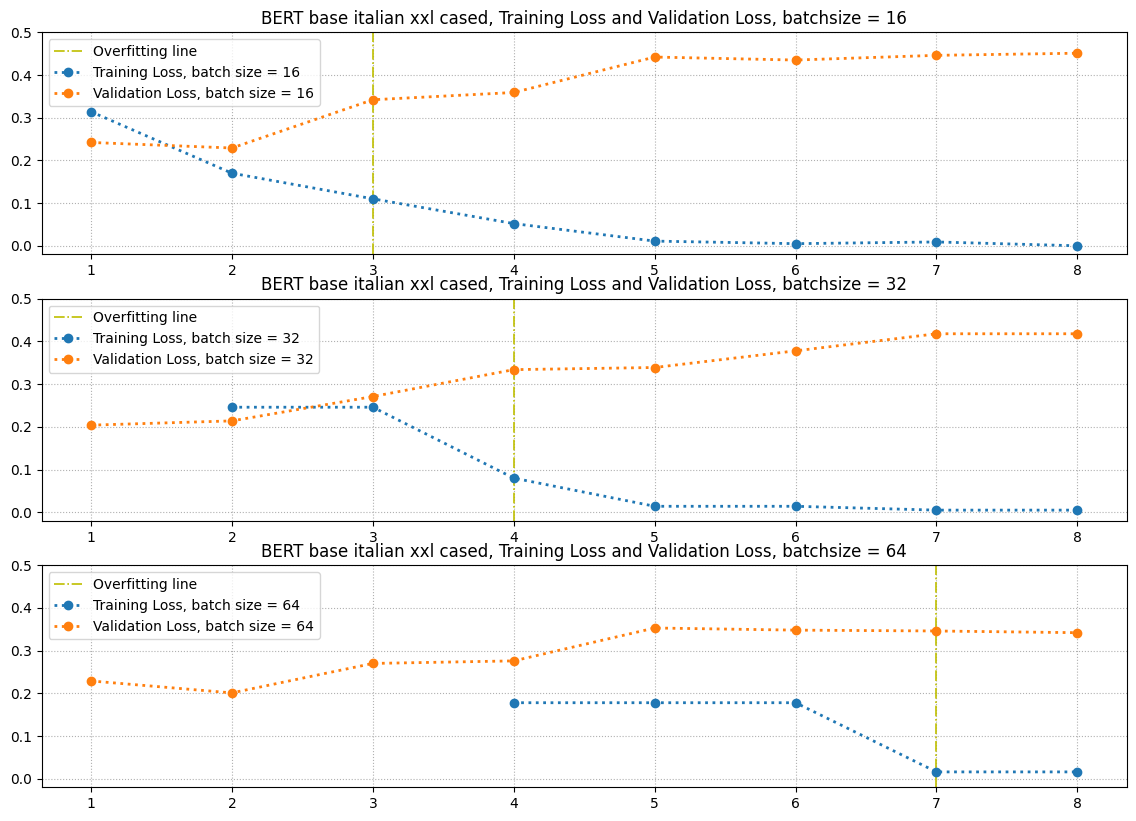
\includegraphics[width=0.65\textwidth]{pics/bert base italian xxl cased/losses xxl.png}
        \caption{BERT base italian xxl cased; risultati funzione obiettivo per il dataset di train e di test}
        \label{fig:losses-xxl}
    \end{figure}
    
    In entrambi i casi i risultati ottenuti riguardo il processo di apprendimento risultano essere molto simili. A seguito di ulteriori prove, aumentando fino a venti il numero di epoche, è possibile generalizzare l'andamento osservato: la probabilità di overfitting si presenta dopo un numero sempre maggiore di epoche proporzionalmente alla dimensione di batch.

\subsection{Metriche sul dataset di test}
    La valutazione del modello, come accennato precedentemente, è stata effettuata sul dataset di test dove ogni commento presente non è mai stato utilizzato per l'apprendimento nelle fasi precedenti. La scelta delle metriche è condizionata da alcuni fattori fondamentali dovuti alla distribuzione delle diverse classi nel dataset stesso. Nello specifico, avendo a disposizione un dataset sbilanciato, non è possibile usare l'accuratezza per descrivere al meglio il comportamento del modello nella fase di classificazione. Prendendo ad esempio il dataset a disposizione con solamente il 15\% di commenti negativi, il modello potrebbe classificare tutti i commenti come positivi e riuscire a raggiungere comunque un livello di accuratezza pari ad un 85\% senza in realtà classificare correttamente nessun commento negativo.
    
    La scelta della metrica ricade quindi sull'F1 score in grado di misurare l'accuratezza di un modello anche in caso di dataset sbilanciato. L'F1 score considera contemporaneamente sia la precisione che il recupero, due metriche utili a capire rispettivamente quanti commenti sono stati classificati correttamente sul totale dei commenti etichettati con una classe dal modello e quanti commenti sono stati correttamente classificati sul numero totale di commenti effettivamente appartenenti a quella classe. In termini più formali la precisione rappresenta il rapporto tra i veri positivi e la somma tra i veri positivi e i falsi positivi; il recupero è invece il rapporto tra i veri positivi e la somma dei vero positivi con i falsi negativi. Il punteggio F1 viene infine calcolato con la media armonica tra precisione e recupero definito di seguito:
    
    \[Precisione = \frac{VP}{VP + FP}\]
    
    \[Recupero = \frac{VP}{VP + FN}\]
    
    \[F_{1} = \frac{2}{\frac{1}{R} + \frac{1}{P}} = 2 \cdot \frac{P \cdot R}{P + R}\]
    
    Le metriche sopra descritte sono rappresentate in figura \ref{fig:f1-uncased} per il modello \textit{BERT base italian uncased} e in figura \ref{fig:f1-xxl} per il modello \textit{BERT base italian xxl cased}.

    \begin{figure}[h]
        \centering
        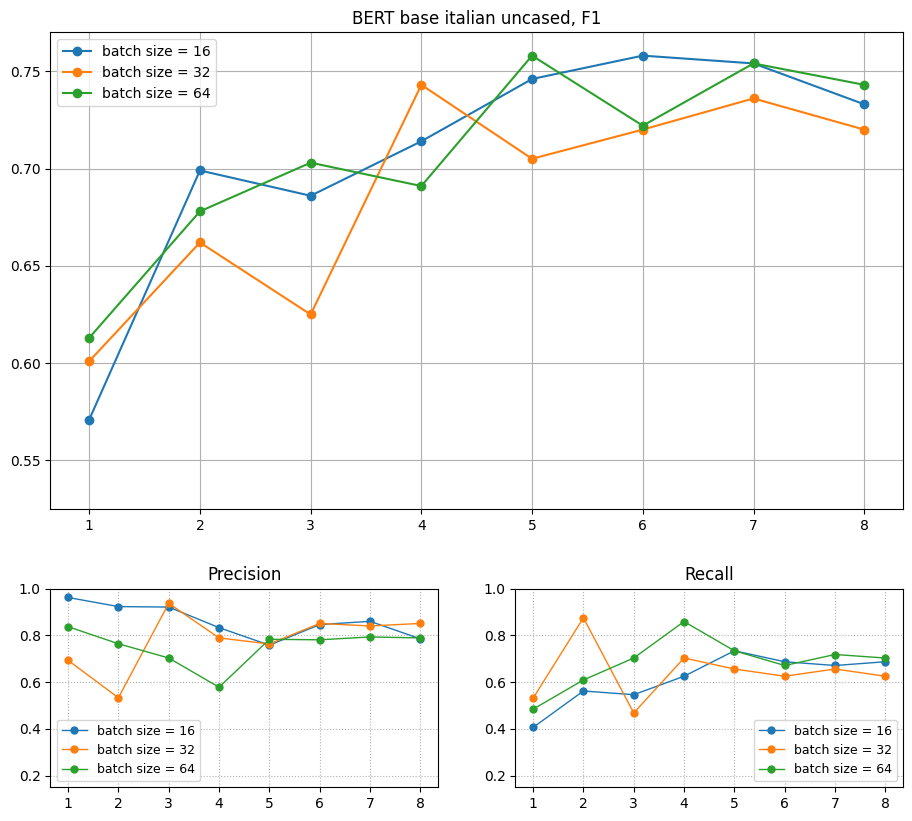
\includegraphics[width=0.8\textwidth]{pics/bert base italian uncased/f1 precision recall.png}
        \caption{\textit{BERT base italian uncased}; F1 score, precisione e recupero}
        \label{fig:f1-uncased}
    \end{figure}
    
    
    \begin{table}[h!]
        \centering
        \begin{tabular}{@{}lcccccc@{}}
        \toprule
                                  & \multicolumn{3}{c}{BERT base italian uncased} & \multicolumn{3}{c}{BERT base italian xxl cased} \\ 
        \multicolumn{1}{c}{Epoch} & 16 batch  & 32 batch   & 64 batch       & 16 batch          & 32 batch   & 64 batch     \\ \midrule
        1                         & 0.571     & 0.601      & 0.613          & 0.606             & 0.660      & 0.666        \\
        2                         & 0.699     & 0.662      & 0.678          & 0.756             & 0.736      & 0.716        \\
        3                         & 0.686     & 0.625      & 0.703          & 0.713             & 0.716      & 0.690        \\
        4                         & 0.714     & 0.743      & 0.691          & \textbf{0.760}    & 0.752      & 0.700        \\
        5                         & 0.746     & 0.705      & \textbf{0.758} & 0.735             & 0.737      & 0.699        \\
        6                         & 0.758     & 0.720      & 0.722          & 0.743             & 0.737      & 0.711        \\
        7                         & 0.754     & 0.736      & 0.754          & 0.735             & 0.728      & 0.733        \\
        8                         & 0.733     & 0.720      & 0.743          & 0.735             & 0.724      & 0.717        \\ \bottomrule
        \end{tabular}
        \caption{Risultati numerici per ogni epoca usando diverse dimensioni di batch}
        \label{Tab:f1-tab}
    \end{table}
    
    Confrontando i risultati ottenuti dai due modelli emerge una leggera superiorità per quanto riguarda il punteggio F1 ottenuto dal modello più grande \textit{BERT base italian xxl cased}. Osservando i valori numerici riportati in tabella \ref{Tab:f1-tab} sono evidenziati i punteggi F1 più alti ottenuti dai due modelli. Se si considera anche il numero di epoche, cercando di preferire il minor numero di iterazioni per evitare overfitting e abbassare i tempi di calcolo, il modello \textit{xxl} si conferma come il migliore tra i due considerati.
    
    \begin{figure}[h!]
        \centering
        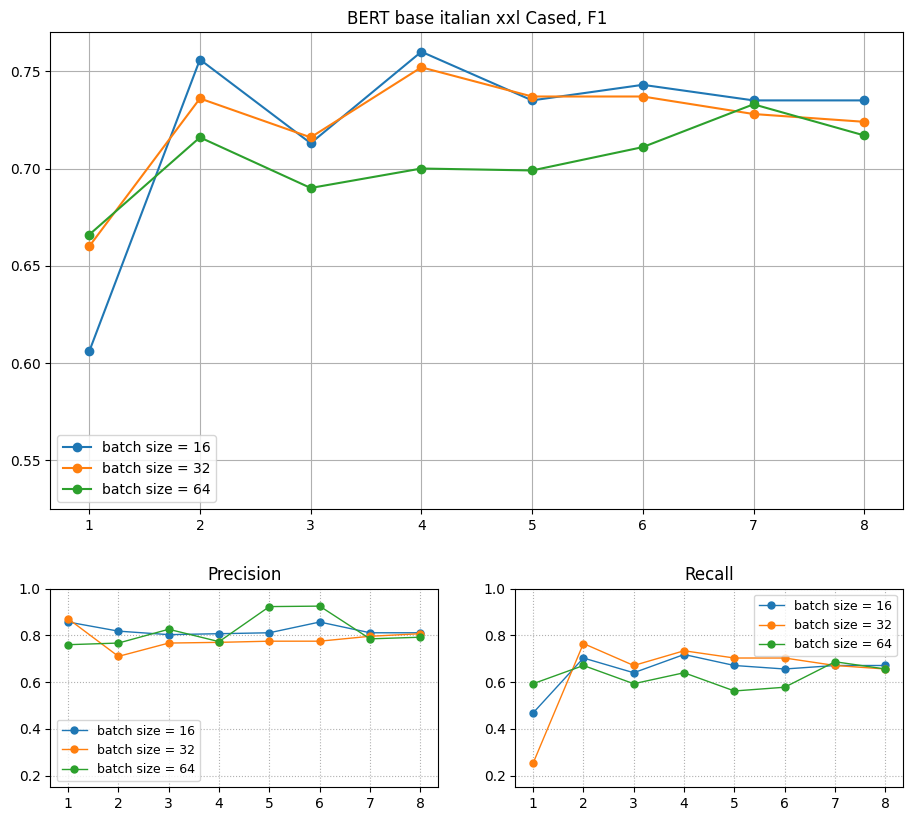
\includegraphics[width=0.8\textwidth]{pics/bert base italian xxl cased/f1 precision recall xxl.png}
        \caption{\textit{BERT base italian xxl cased}; F1 score, precisione e recupero}
        \label{fig:f1-xxl}
    \end{figure}
    
    La libreria PyTorch permette il salvataggio dei pesi trovati durante il processo di fine tuning del modello. Ricostruendo la rete neurale e importando i pesi precedentemente calcolati è possibile svolgere alcuni test manuali per osservare da più vicino il comportamento del modello nei diversi scenari di utilizzo. Le frasi più banali, la cui classe di appartenenza è ovvia anche con un semplice controllo del lessico, vengono classificate correttamente senza problemi mantenendo una probabilità restituita dalla funzione sigmoidea generalmente superiore al 85\%. Per mettere in difficoltà il modello è quindi necessario usare frasi che condividono lo stesso tipo di linguaggio ma con un significato diametralmente opposto. L'esempio riportato nella tabella \ref{Tab:class-example} mostra il risultato restituito dal modello in entrambi i casi. Nel secondo esempio è evidente come BERT non svolga solo un ruolo di classificazione basato sui termini utilizzati ma riesce efficacemente a comprendere il loro contesto di utilizzo interpretando correttamente il senso della frase. Viene ulteriormente segnalato come il problema dell'unintended bias nella classificazione dei discorsi d'odio (presentato e studiato in \cite{FersiniBias}) risulta essere efficacemente gestito dalla rete neurale testata.
    
    Rimane comunque importante sottolineare che la buona precisione riscontrata negli esempi riportati è dovuta alla forte presenza di termini simili nel dataset di train che permettono quindi un apprendimento efficace del modello stesso. Lo stesso comportamento non è sempre osservabile se si utilizzano vocaboli non presenti nel dataset di train dimostrando come, sopratutto quando si parla di reti neurali profonde, una grande quantità di dati risulta essere indispensabile per ottenere un modello che riesca a mantenere delle buone prestazioni anche nel mondo reale.
    
    \begin{table}[h]
        \centering
        \begin{tabular}{@{}lllc@{}}
        \toprule
          & \multicolumn{1}{l}{Commento} & Classe    & \multicolumn{1}{l}{Output funzione sigmoidea} \\ \hline %\cmidrule(l){1-4} 
        1 & \textit{Sei bravissima, complimenti}    & Good      &   0.06    \\
          & \textit{Sei bruttissimo, vergognati}    & Offensive &   0.97    \\
        \\
        2 & \textit{Dai, povero...}                  & Good      &   0.38    \\
          & \textit{Sei un povero}                  & Offensive &   0.78    \\ \bottomrule
        \end{tabular}
        \caption{Esempi di classificazione manuale per verificare la comprensione del contesto del modello BERT}
        \label{Tab:class-example}
    \end{table}
    
    
\section{Modifiche al modello BERT base}
I risultati ottenuti con l'utilizzo del modello base di BERT sono più che soddisfacenti per un semplice task di classificazione ma è possibile migliorare il risultato ottenuto aggiungendo dei layer che, invece di considerare l'output della classificazione (o pooler layer), raccolgono l'output dell'ultimo layer di BERT (768 nodi) e continuano il processo di fine-tuning.

Come accennato nel \hyperref[sec:FrameworkProposto]{capitolo relativo framework proposto} vengono proposte due modifiche diverse al modello BERT di base. La prima riguarda l'aggiunta di un layer di tipo Bi-LSTM in grado di memorizzare gli input antecedenti e seguenti, caratteristica peculiare delle reti neurali ricorrenti; la seconda riguarda l'aggiunta di un layer lineare, uno di dropout e infine un ultimo layer di output in grado di classificare nelle due classi gli input ricevuti. 

Come banchmark per il confronto delle prestazioni viene scelto il modello con i migliori risultati trovati nei capitoli precedenti: \textit{BERT base italian xxl cased} con una dimensione di batch pari a 16.

\subsection{BERT con layer Bi-LSTM}
    La prima modifica apportata al modello è stata aggiungere un layer Bi-LSTM in coda a BERT. Durante la fase di addestramento, osservando i risultati della funzione obiettivo per il dataset di train e di test in figura \ref{fig:bert-bi-lstm}, si può notare come i valori della loss function sul dataset di test aumentino dopo ogni epoca segnalando la probabile occorrenza di un problema di overfitting. Contemporaneamente la performance del modello, rappresentata dalla spezzata a destra, misurata dal punteggio F1 è in leggera discesa ma riesce a mantenere comunque dei valori in linea, o di poco inferiori, rispetto a quelli visti dal modello base di BERT.
    
    
    \begin{figure}[h]
        \centering
        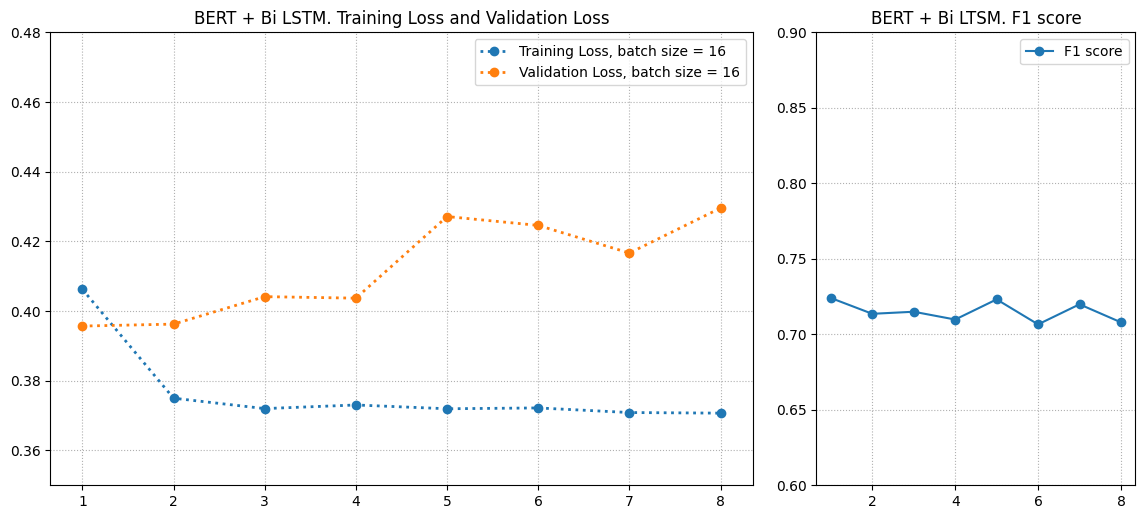
\includegraphics[width=0.8\textwidth]{pics/modifiche bert/BERT Bi LSTM.png}
        \caption{Metriche del modello BERT base con un layer Bi-LSTM in coda}
        \label{fig:bert-bi-lstm}
    \end{figure}
    
    
    A fronte di una validation loss maggiore e un punteggio F1 quasi identico al modello base di BERT è possibile concludere che questa modifica effettuata, almeno in questo caso, non porti a nessun vantaggio effettivo rispetto all'impiego del modello base. Questo comportamento è probabilmente attribuibile alla struttura delle reti neurali ricorrenti spiegate nel capitolo relativo al framework proposto. La loro capacità di ricordare è ristretta ai token vicini (destra e sinistra nel caso di una LSTM bidirezionale) e risulta essere quindi limitante rispetto all'ottima capacità di encoding di un'intera frase da parte delle reti neurali di tipo transformer di cui BERT fa parte.

\subsection{BERT con layer lineare, dropout e di classificazione}
    In figura \ref{fig:bert-linear} vengono rappresentati i risultati ottenuti dalla seconda modifica effettuata al modello base di BERT. In questo caso sono state effettuate diverse prove prima di ottenere il miglior risultato possibile. Inizialmente era stato utilizzato un singolo layer denso dimostratosi però inefficace nel migliorare le performance a causa del presentarsi di overfitting già dalla prima epoca. Si è quindi scelto di introdurre un layer di regolarizzazione, più nello specifico di dropout, per cercare di mitigare il problema di overfitting e subito dopo un semplice layer di classificazione in grado di restituire valori compatibili con le due classi dei commenti. Dopo diversi tentativi si è trovata la miglior percentuale di dropout fissata a 0.2. 
    
    \begin{figure}[h]
        \centering
        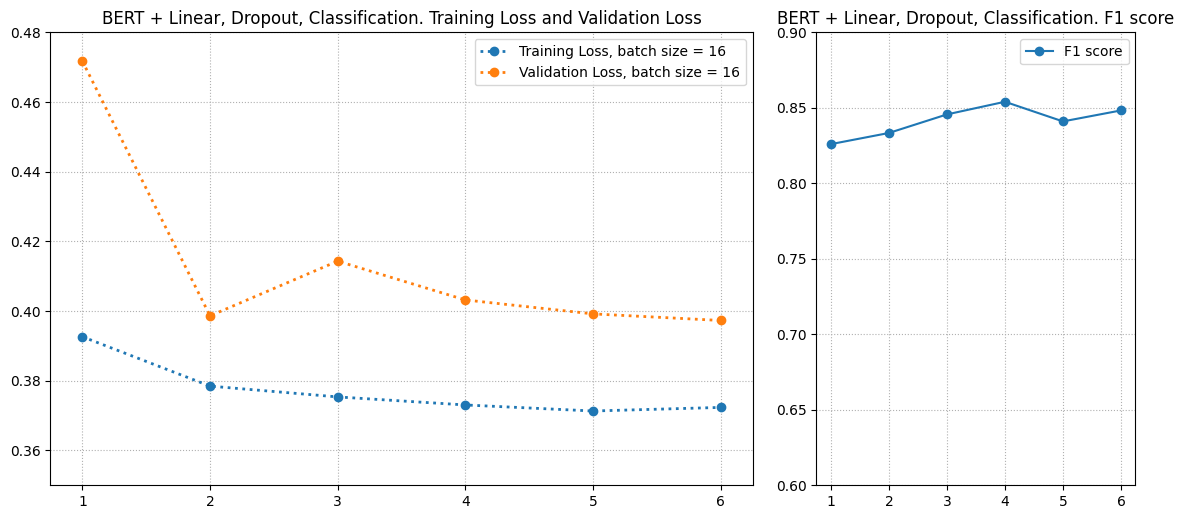
\includegraphics[width=0.8\textwidth]{pics/modifiche bert/BERT Linear.png}
        \caption{Metriche del modello BERT base con un layer lineare e uno di dropout in coda}
        \label{fig:bert-linear}
    \end{figure}
    
    I dati di classificazione ottenuti dimostrano come, nonostante una validation loss più alta della training loss in fase di training, le metriche sul dataset di test rimangano più che accettabili nel corso delle epoche. È possibile supporre che, in presenza di un dataset più grande nella fase di addestramento, i risultati della funzione obiettivo sarebbero stati sicuramente migliori: la rete neurale, con anche l'aggiunta dei nuovi layers visti precedentemente, risulta essere troppo grande per una quantità di dati così bassa.
    
\subsection{Confronto risultati con le modifiche effettuate}

    Viene infine proposto un grafico riassuntivo in figura \ref{fig:f1-comp-f} dove vengono illustrati i diversi punteggi F1 ottenuti sia dal modello base di BERT sia dai modelli con le modifiche apportate. Tra tutti i modelli proposti il migliore risulta essere BERT con i layer lineari e di dropout aggiunti in coda. Come anticipato il modello BERT base e il modello BERT con l'aggiunta di un layer Bi-LSTM si mantengono sulle stesse performance con un leggero vantaggio per il secondo a fronte però di una validation loss più alta vista precedentemente.
    
    
    \begin{figure}[h]
        \centering
        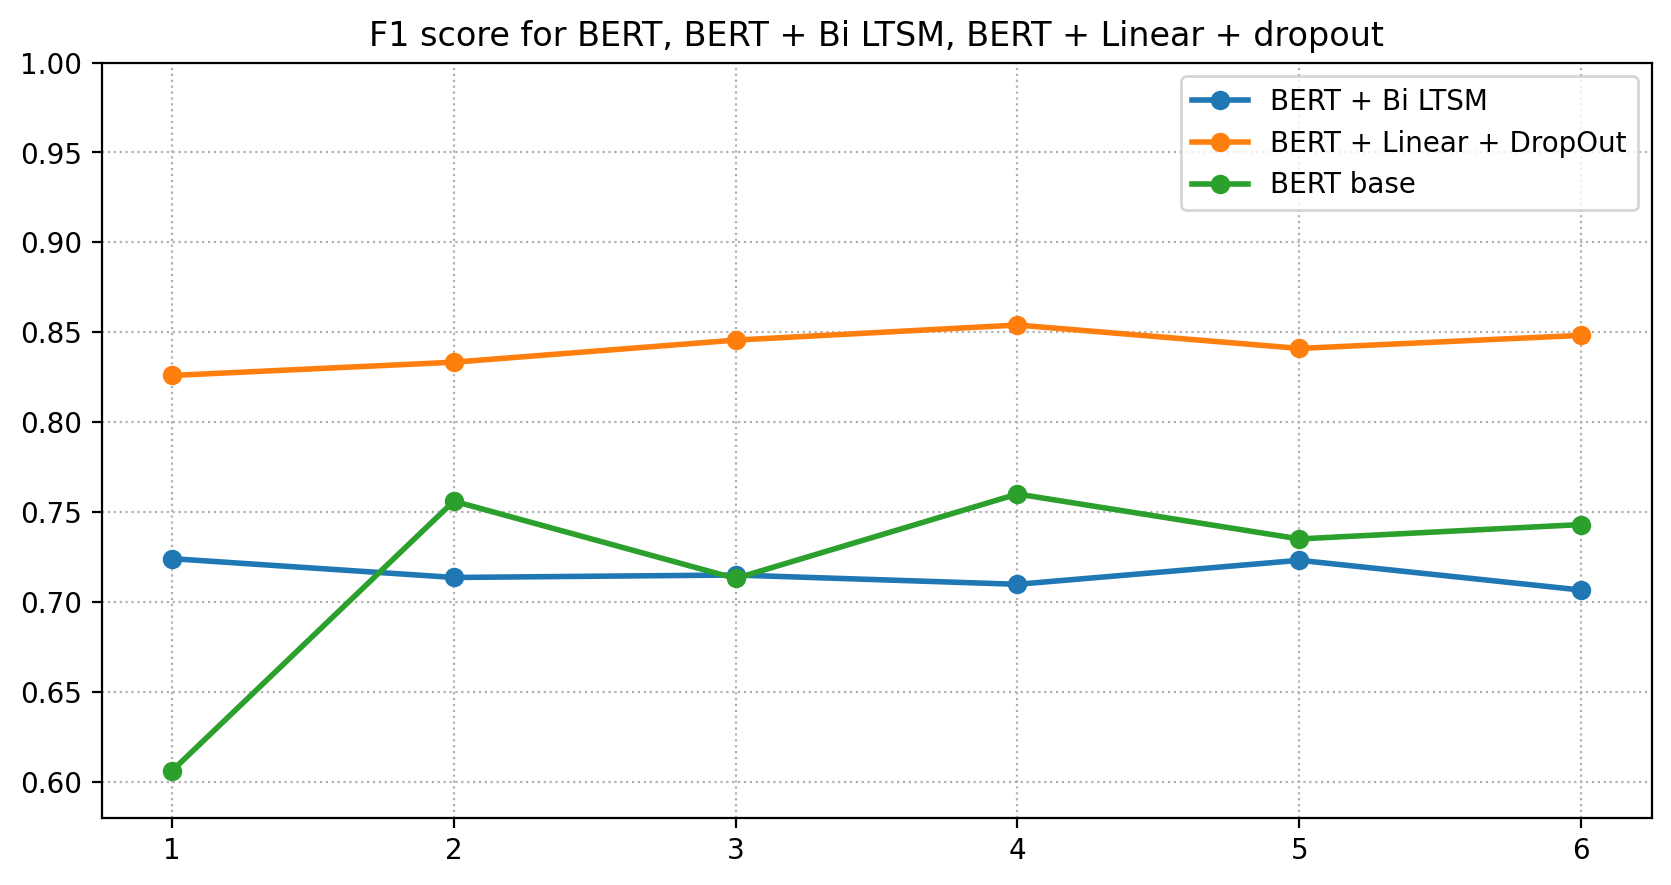
\includegraphics[width=0.8\textwidth]{pics/modifiche bert/F1 BERT Bi LSTM Linear stretched.png}
        \caption{Risultati ottenuti dal miglior modello BERT base e dai modelli modificati con i layer aggiuntivi}
        \label{fig:f1-comp-f}
    \end{figure}
    
    
    Nella tabella riepilogativa \ref{Tab:f1-comp-t} sono vengono ulteriormente riportati i punteggi F1 relativi alla prima classificazione con il lessico Hurtlex. Come previsto da una prima ispezione manuale, il lessico non è stato in grado di classificare efficacemente i commenti offensivi ottenendo un punteggio decisamente più basso dei modelli analizzati.
    
    \begin{table}[h]
    \begin{tabular}{@{}lcccccc@{}}
        \toprule
        Epoch & \begin{tabular}[c]{@{}c@{}}BERT\\ base\end{tabular} & \begin{tabular}[c]{@{}c@{}}BERT\\ Bi-LSTM\end{tabular} & \begin{tabular}[c]{@{}c@{}}BERT\\ Linear\\ dropout\end{tabular} & Hurtlex & \begin{tabular}[c]{@{}c@{}}Hurtlex\\ only\\ conservative\end{tabular}\\ \midrule
        %Epoch & BERT base & BERT + Bi-LSTM & BERT + Linear + dropout & Hurtlex   & Hurtlex only cons\\ \midrule
        1     & 0.606     & 0.724          & 0.825                   & -          & -           \\
        2     & 0.756     & 0.713          & 0.833                   & -          & -           \\
        3     & 0.713     & 0.714          & 0.845                   & -          & -           \\
        4     & 0.760     & 0.709          & \textbf{0.853}          & -          & -           \\
        5     & 0.735     & 0.723          & 0.840                   & -          & -           \\
        6     & 0.743     & 0.706          & 0.848                   & -          & -           \\ 
              & -         & -              & -                       & 0.121      & 0.154       \\\bottomrule
    \end{tabular}
    \caption{Tabella riepilogativa dei migliori risultati numerici ottenuti con tutti i metodi di classificazione utilizzati}
    \label{Tab:f1-comp-t}
    \end{table}
    
    
    